\section{Limitations}

Despite the success of the final YOLOv11s pipeline, several limitations must be 
acknowledged regarding the data, the modeling approach, and the downstream application 
of the system.

\textbf{Imaging and Dataset Constraints}

First, the $352 \times 240$ resolution of the 511NY and NYSDOT camera feeds places
a clear limit on how much visual detail the detector can use. Many vehicles appear 
too small, too blurry, or too occluded to classify confidently, which is reflected
in the dataset by the large number of \verb|unknown_vehicle| annotations. This low 
resolution is helpful from a privacy standpoint, since it makes license plates and 
faces effectively unreadable, but it also makes the system less reliable for smaller
or farther vehicles. In addition, the camera imagery itself is not always consistent.
As shown in Figure~\ref{fig:camera-no-feed}, some cameras occasionally produce degraded 
frames due to servicing, feed glitches, motion blur, or strong lighting effects. 
Nighttime glare (Figure~\ref{fig:camera-artifact-a}), 
direct sunlight striking (Figure~\ref{fig:camera-artifact-b}), 
and image corruption (Figure~\ref{fig:camera-artifact-c})
can all reduce visibility and make vehicle boundaries harder to distinguish. These 
imaging inconsistencies introduce an additional source of noise that cannot be fully 
controlled during training.

\begin{figure}[!htbp]
    \centering
    \begin{subfigure}[t]{0.32\textwidth}
        \centering
        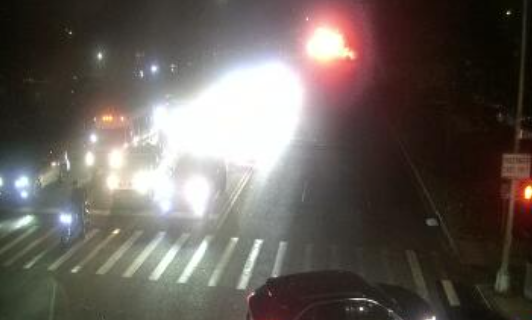
\includegraphics[width=\textwidth]{figures/limitations/7_night_glare.png}
        \caption{Nighttime overexposure and glare}
        \label{fig:camera-artifact-a}
    \end{subfigure}
    \hfill
    \begin{subfigure}[t]{0.32\textwidth}
        \centering
        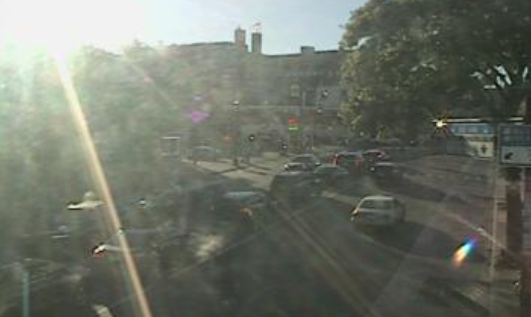
\includegraphics[width=\textwidth]{figures/limitations/7_sun_glare.png}
        \caption{Daytime sun glare and lens flare}
        \label{fig:camera-artifact-b}
    \end{subfigure}
    \hfill
    \begin{subfigure}[t]{0.32\textwidth}
        \centering
        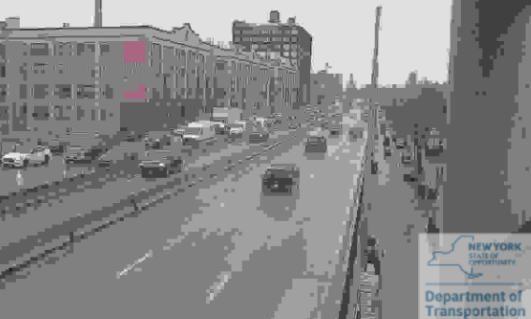
\includegraphics[width=\textwidth]{figures/limitations/7_glitched_frame.png}
        \caption{Degraded camera feed with image corruption}
        \label{fig:camera-artifact-c}
    \end{subfigure}
    \caption{Examples of image-quality issues observed in the 511NY and NYSDOT traffic-camera feeds. These artifacts reduce visibility and make vehicle boundaries harder to distinguish during annotation and detection.}
    \label{fig:camera-artifacts}
\end{figure}

Furthermore, although the training set contains 1,200 unique images, it was drawn 
from only 12 camera intersections, with more than half located in Manhattan and 
fewer examples from other boroughs such as the Bronx and Queens. In addition, because 
these are Pan-Tilt-Zoom (PTZ) cameras, their viewpoints are not fixed, so the dataset 
does not represent every viewing angle that may occur in practice. This could help 
explain why performance dropped on the unseen-camera benchmark, as the model learned
the original camera set well, but generalized less reliably to new views. Class 
imbalance was another important limitation. Some categories, especially \verb|motorcycle|, 
were represented by very few examples in training. With only 49 labeled motorcycles, 
that class had the weakest test-set performance and was often visually confused with 
bicycles or other small two-wheeled objects.

% ------------------------------------------------------------------------------


